\documentclass[]{beamer}
\usepackage[utf8]{inputenc}
\usepackage{graphicx}
\usetheme{Copenhagen}
\usecolortheme{seahorse}

\title{Implementacija osnovnih git komandi}
\author{Adrian Bralic Toth \and Anton Frlan}
\institute{Tehnički Fakultet Rijeka}
\date{2018}

\begin{document}

\frame{\titlepage}

\begin{frame}{git init}

\begin{itemize}
	\setlength\itemsep{1em}
	\item git init stvori .git datoteku te ostale u njoj napravi jos neke datoteke potrebne za rad git-a
	\begin{figure}[scale=.48]
\centering
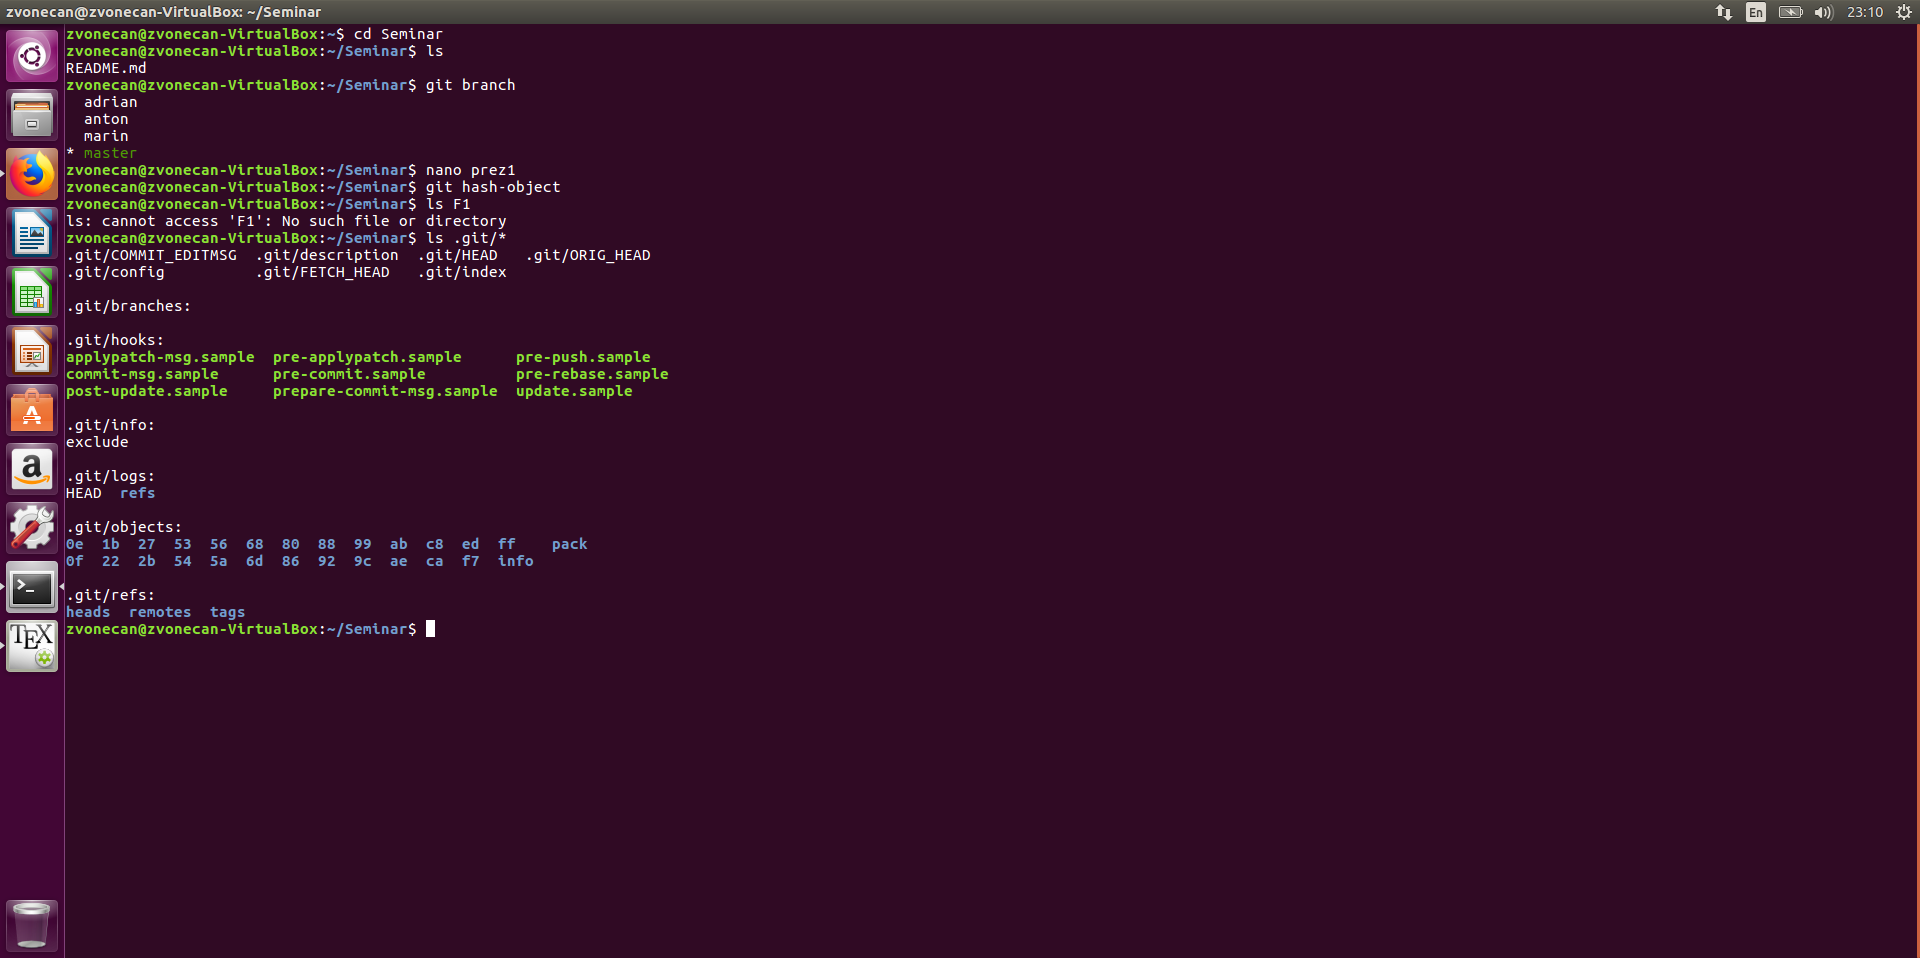
\includegraphics{./slike/git_datoteka.png}
\end{figure}
\end{itemize}

\end{frame}


\begin{frame}{git commit}

\begin{itemize}
	\setlength\itemsep{1.5em}
	\item git commit git izvrsava tako da datoteku spremi pod kljuc zvan SHA-1
	\item SHA-1 je kombinacija od 40 malih slova ili brojeva koja sluzi kao pointer na spremljenu datoteku
	\item pomocu komande git hash-object mozemo spremi neki file u git te dodavanjem -w nam git vraca SHA-1 od tog file-a
	\begin{figure}[scale=.48]
\centering
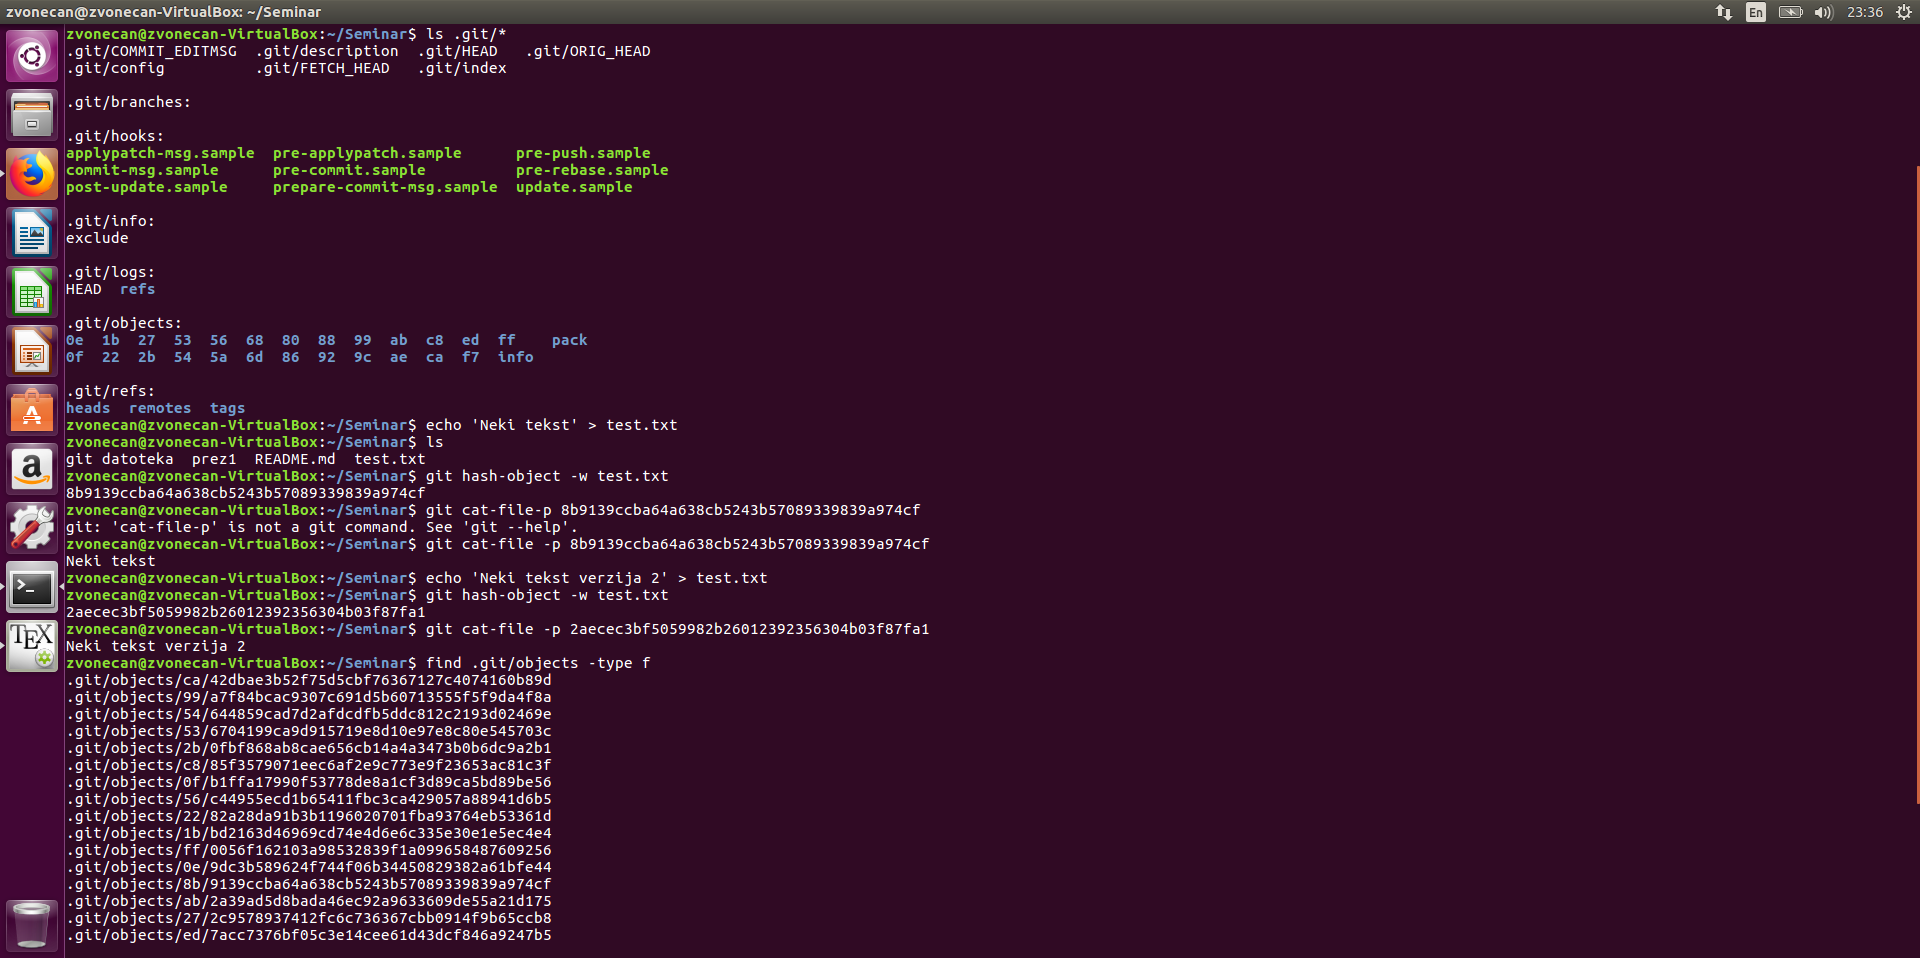
\includegraphics{./slike/druga_slika.png}
\end{figure}
	\item pomocu git hash-object spremamo neki file pod SHA-1 kao blob i mozemo mu pristupiti samo pomocu SHA-1 kljuca
\end{itemize}

\end{frame}


\begin{frame}{git commit}

\begin{itemize}
	\item git rjesava taj problem pomocu stabala
	\item blob je neki podatak / tekst dok je stablo vise bloboa i barem 1 stablo od kojih 1 stablo ima SHA-1 te datoteke ili stabla koji ga ima
	\begin{figure}
		\centering
	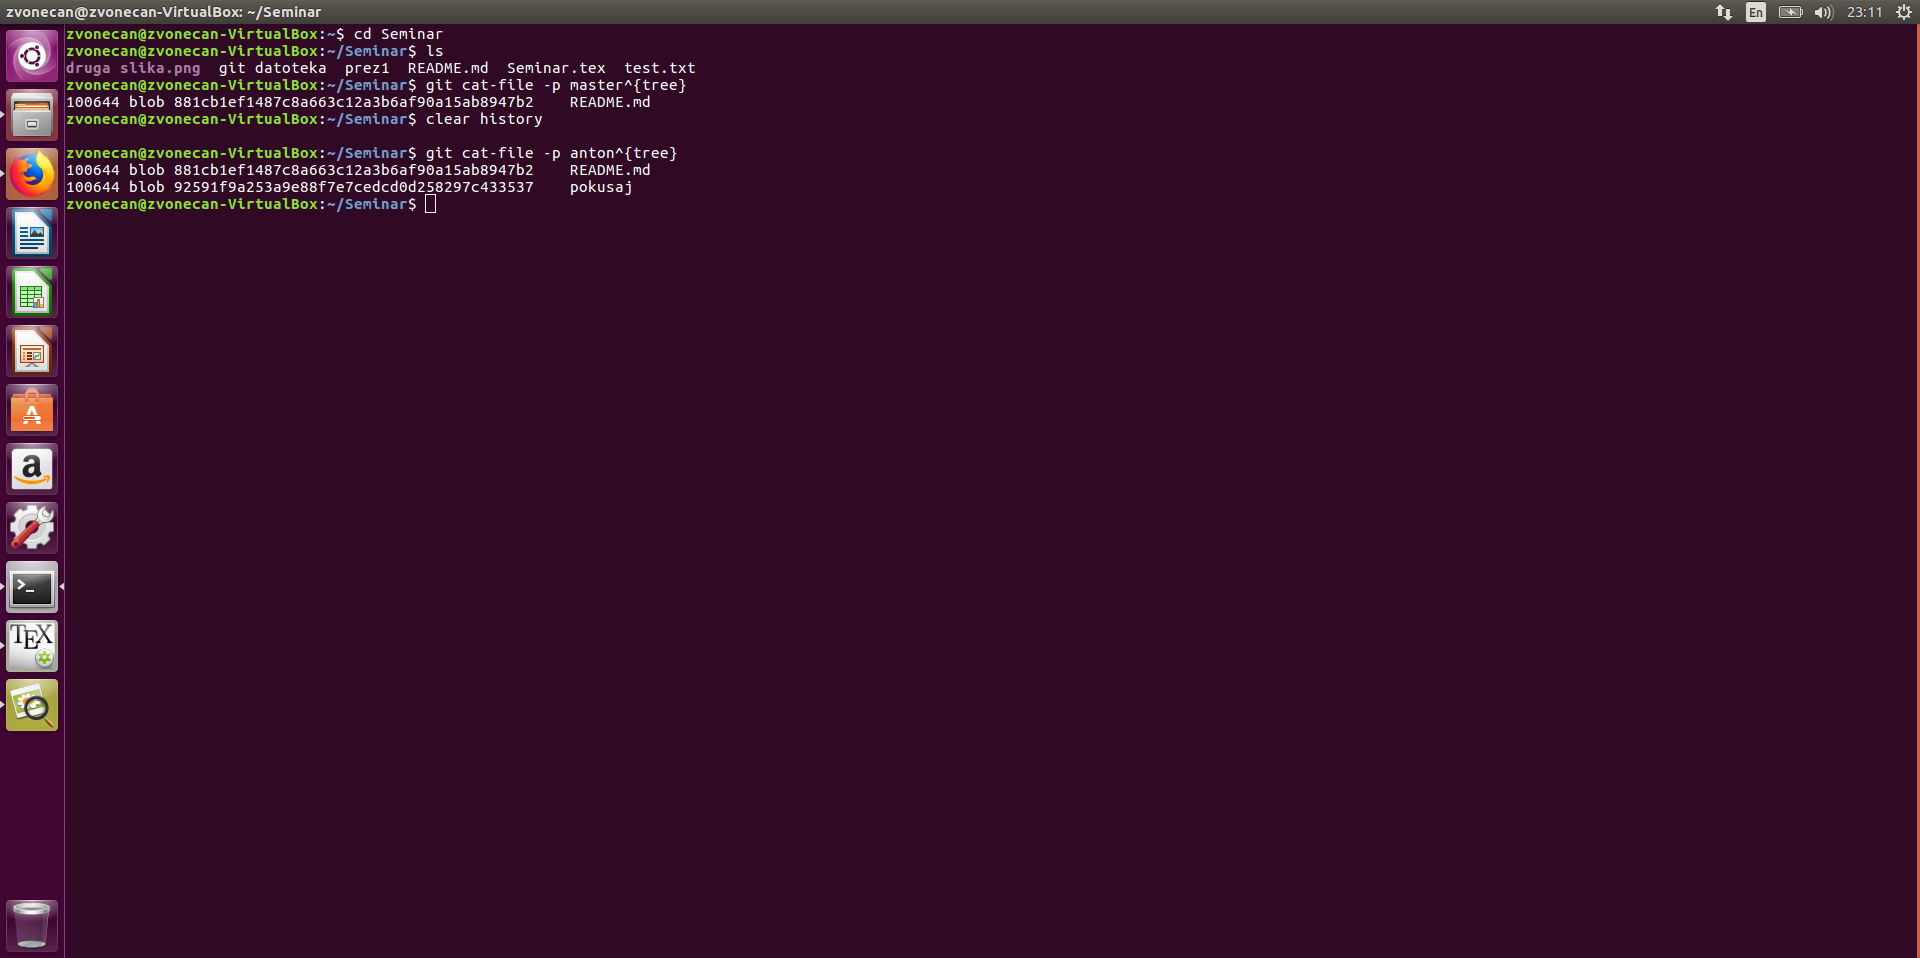
\includegraphics[scale=.48]{./slike/treca_slika.png}
	\end{figure}
	\item kada git commita file on obicno uzme sto je na stage-u i spremi u jedno stablo ili kombinaciju stabla koji su svi spremljeni pod jedno stablo
\end{itemize}
\end{frame}

\begin{frame}{git stage}

\begin{itemize}
	\item file u gitu stage-amo tako da ga dodamo u pod datoteku index unutar .git datoteke
	\item file dodajemo u index pomocu git update-index --add
	\begin{figure}
		\centering
	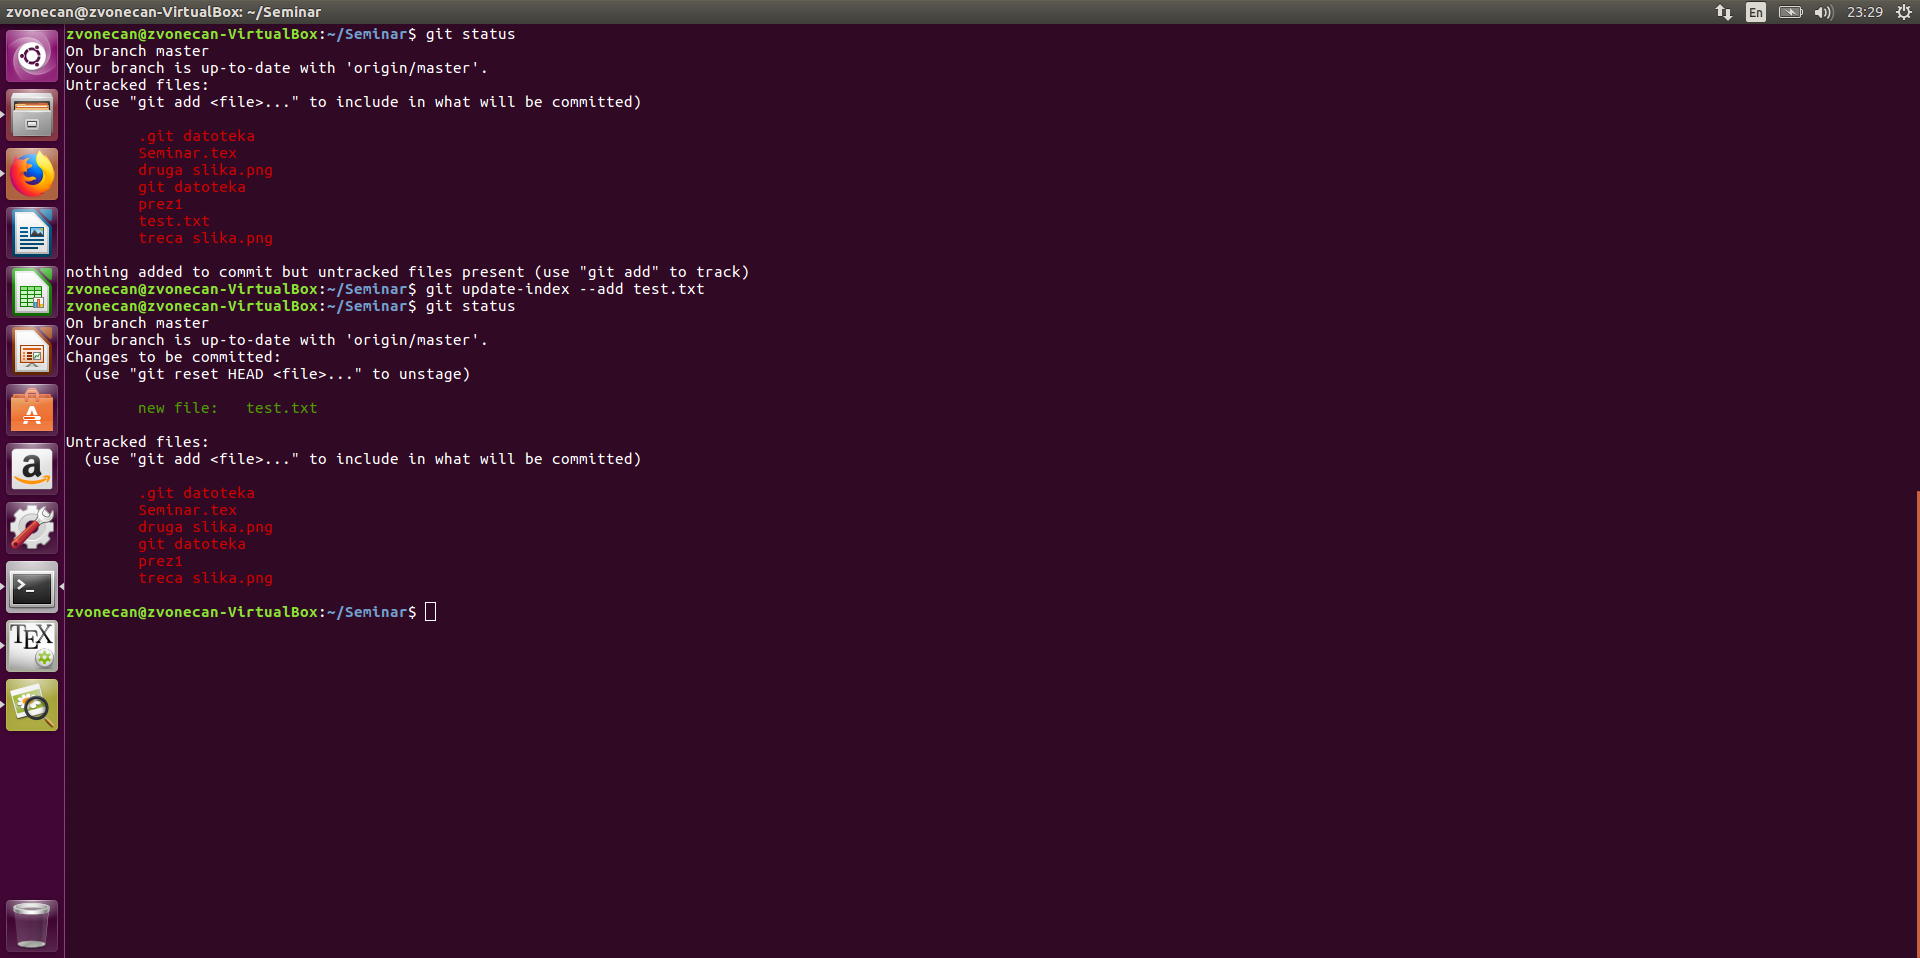
\includegraphics[scale=.48]{./slike/cetvrta_slika.png}
	\end{figure}
	\item ako zelimo stage-a neki prijasnji commit prije imena file-a moramo doda --cached i SHA-1 tog file-a
	\item sad mozemo napraviti istu stvar sto git radi sa file-ovima u indexu , stablo
	\begin{figure}
		\centering
	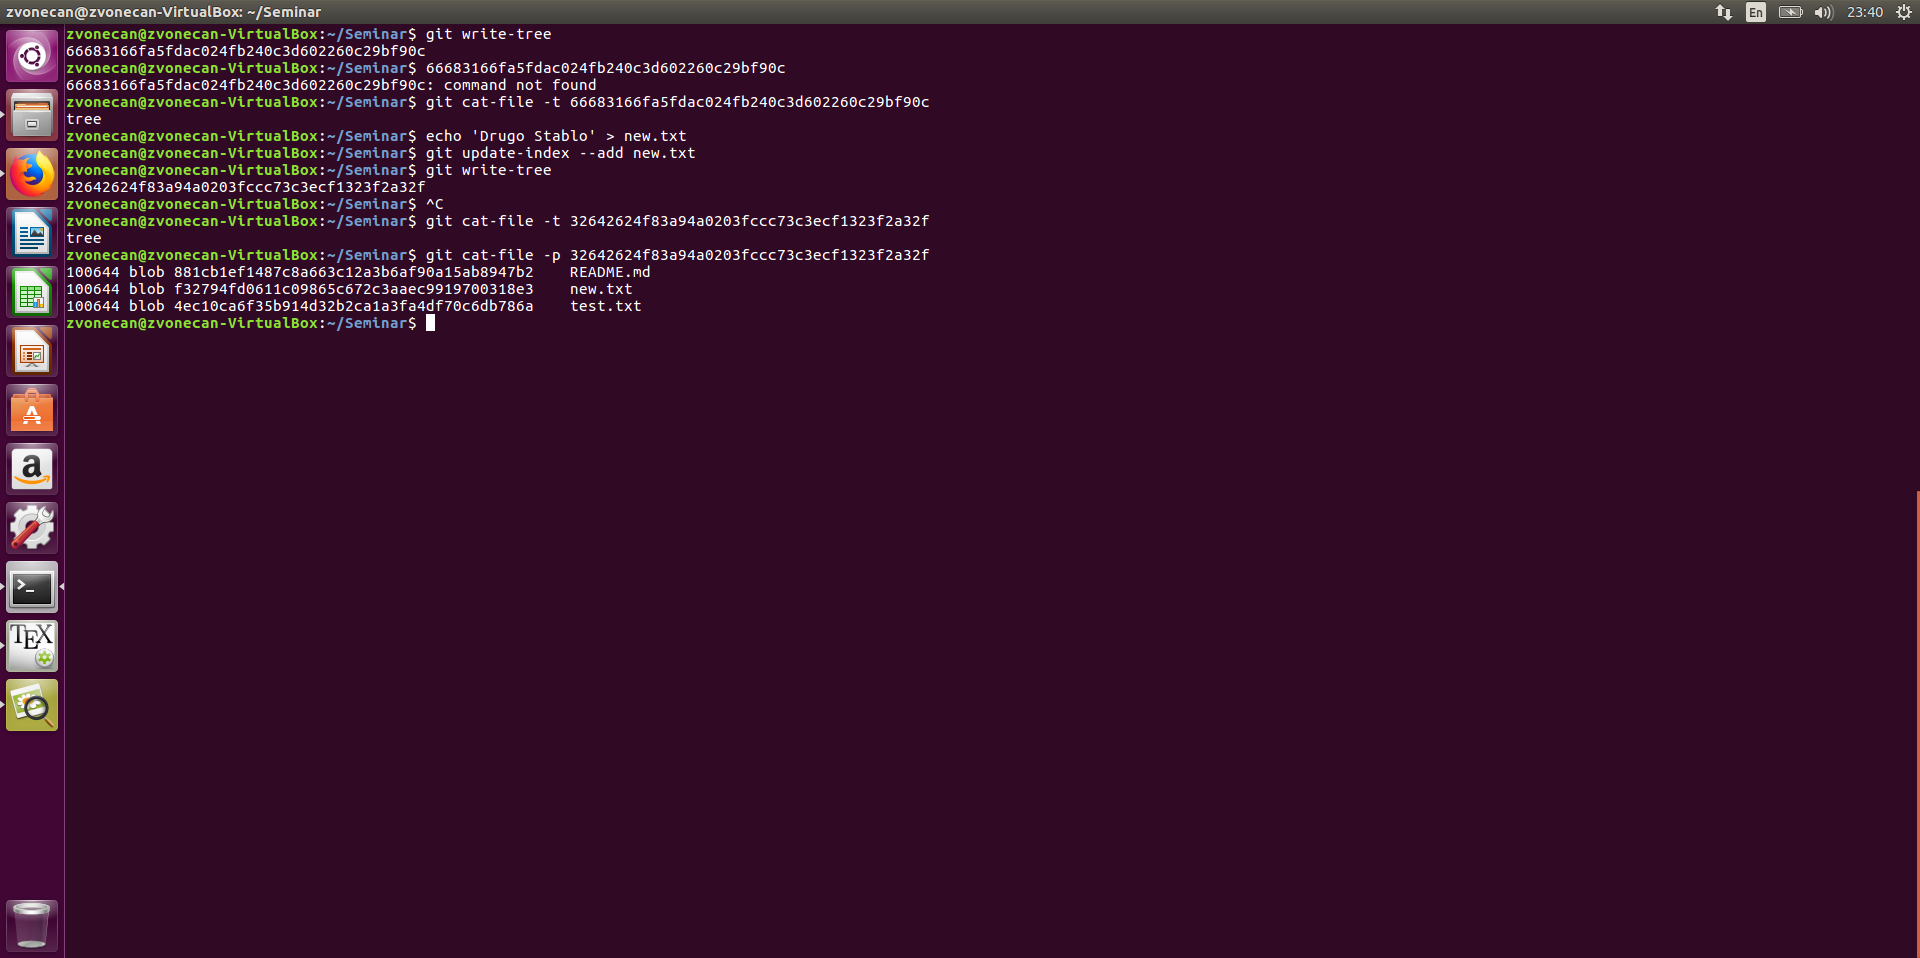
\includegraphics[scale=.48]{./slike/peta_slika.png}
	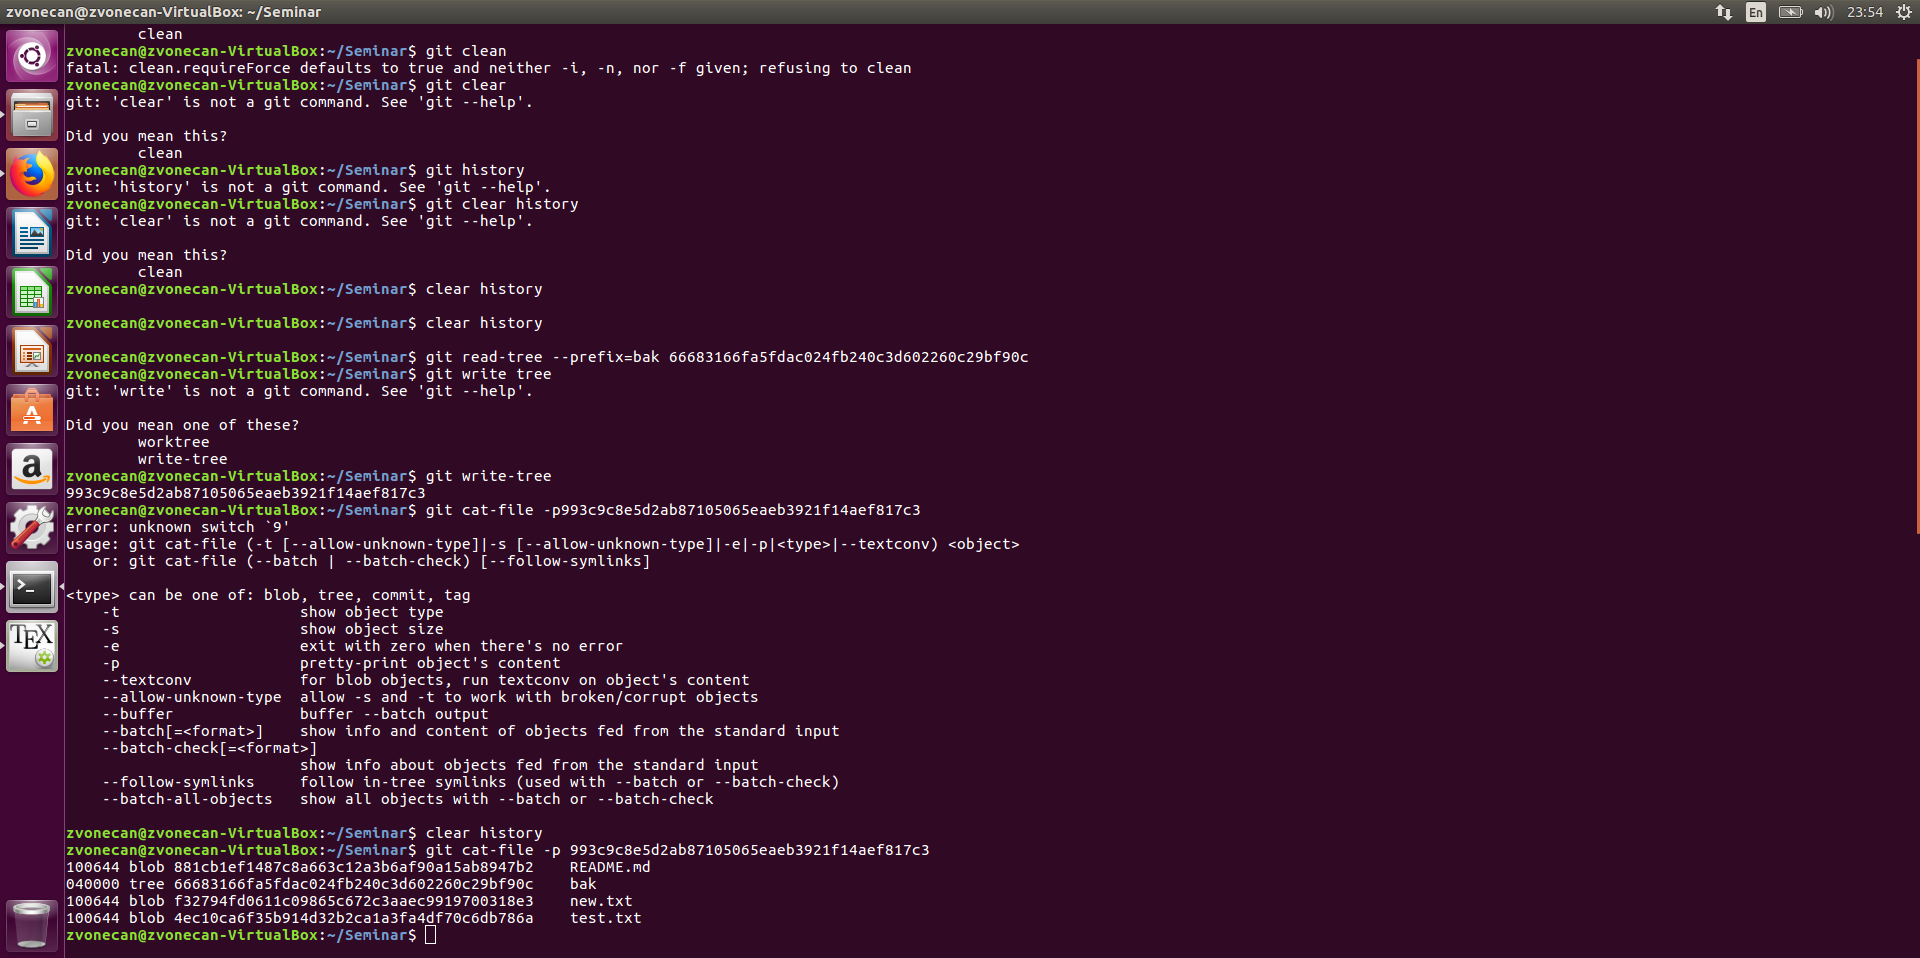
\includegraphics[scale=.48]{./slike/sesta_slika.png}
	\end{figure}
		
\end{itemize}


\end{frame}
\begin{frame}{git commit}

\begin{itemize}
	\item sad samo commitamo stablo koje smo napravili te smo izvrsili istu stvar koju git napravi kada nesto add-amo i commit-amo
	\begin{figure}
		\centering
	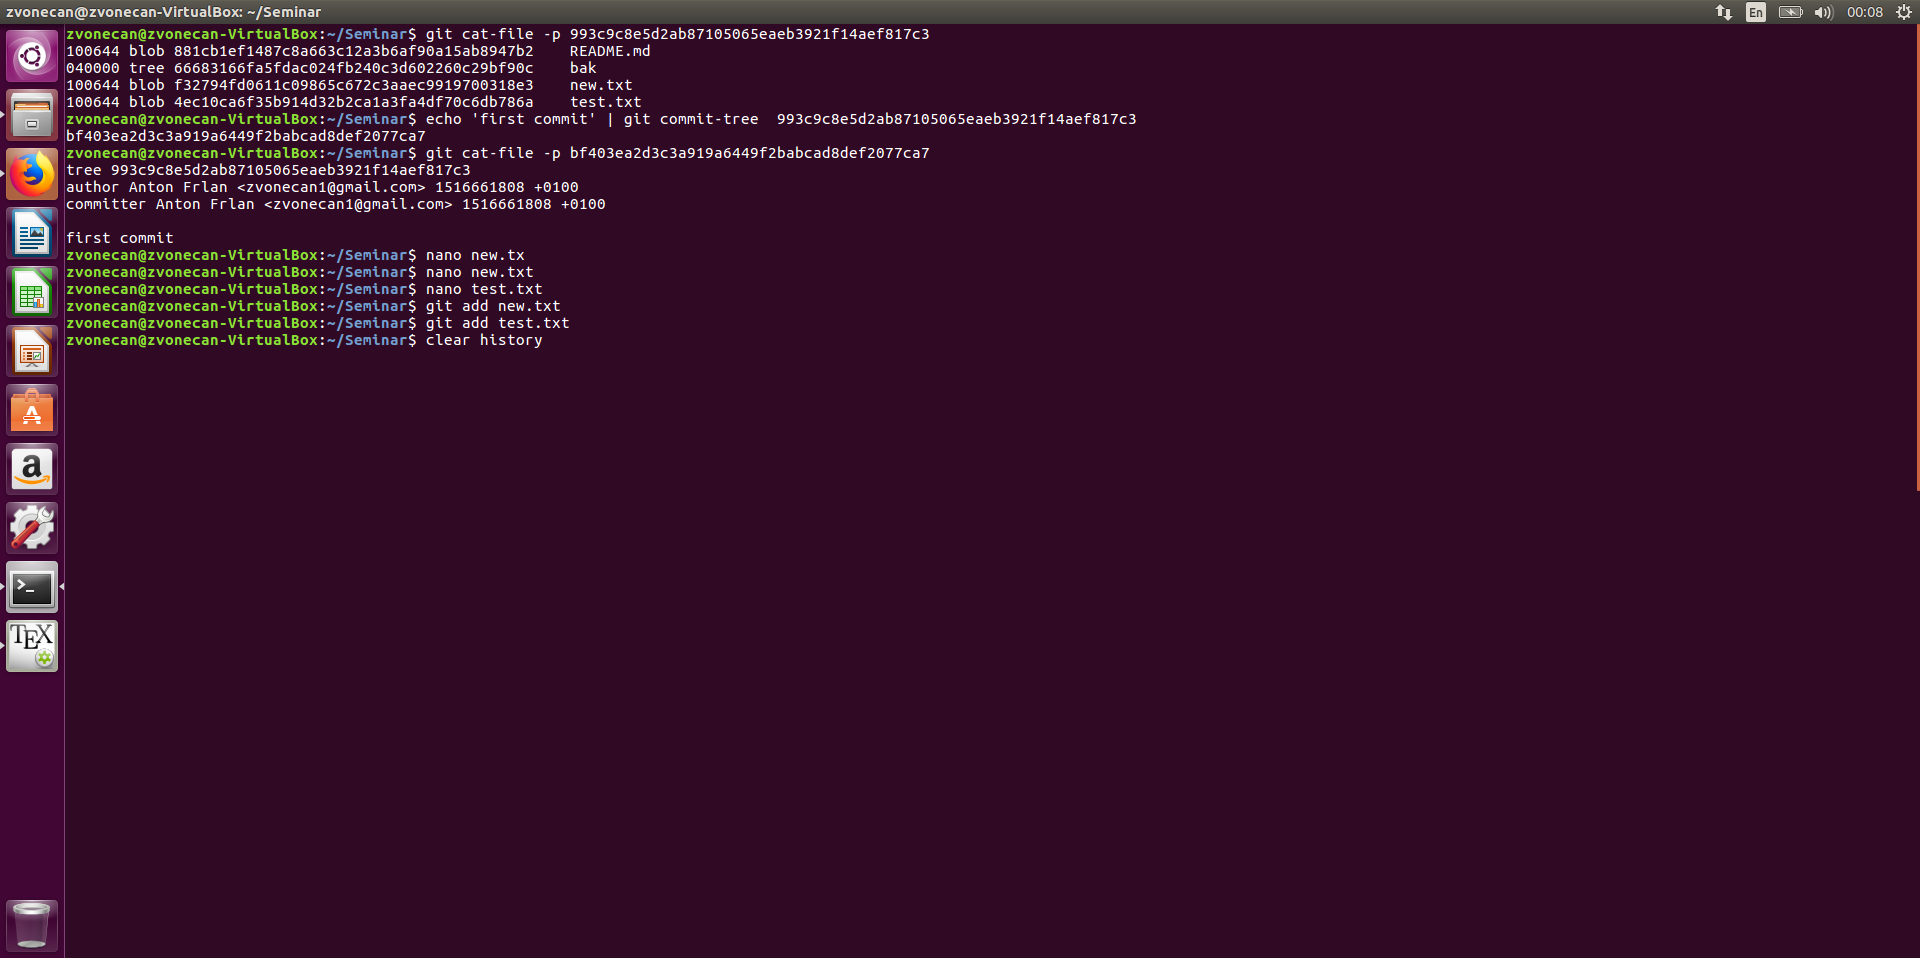
\includegraphics[scale=.48]{./slike/sedma_slika.png}
	\end{figure}
\end{itemize}
\end{frame}

\end{document}